\chapter[Referencial Teórico]{Referencial Teórico}

Neste capítulo, serão abordados conceitos que são imprescindíveis para a compreensão do trabalho em questão.

\section{Mercado de Moedas}

\subsection{Análise Técnica}
Existem dois tipos principais de análises no Mercado de Moedas, análise fundamental e análise técnica.\cite{kumar}

Análise fundamental é baseada no sentido de que acontecimentos mundiais tem impacto direto e são refletidos depois de algum tempo no mercado de moedas, assim sendo,
negociadores podem tirar proveito disso e trocar moedas baseando em por exemplo, notícias a respeito de algum país, entendendo o mercado
mundial como um todo e sabendo evidenciar os acontecimentos que terão algum impacto no Mercado de Moedas. Exemplos de notícias que afetam
o Mercado de Moedas são notícias a respeito de recursos.\cite{baresa}

Análise técnica é a análise em que este trabalho se baseia, e parte do pressuposto que toda a informação refletida no Mercado de Moedas está
contida no preços dos pares. Este tipo de análise se baseia principalmente na análise dos gráficos e indicadores, acreditando que se toda
informação está contida nos gráficos, não é necessário analisar notícias, acontecimentos e o calendário econômico por exemplo. Análise técnica
se encaixa mais neste estudo por ser mais precisa, enquanto a análise fundamental se baseia no próprio conhecimento do negociador, podendo muitas
vezes ser uma opinião subjetiva deste. A análise técnica busca evidenciar padrões e regras para tentar prever os movimentos do mercado. \cite{taylor}

\subsection{Tendência}

Analisando um gráfico do mercado de moedas, pode-ser observar algumas vezes claramente, outras não, o conceito de tendência que nada mais é
do que o sentido geral em que um par de negociação está se movimentando.\cite{werner}

Na figura 01 consegue-se observar o sentido claramente, sabendo que o valor do par está aumentando em função do tempo.
Em alguns casos é mais difícil saber qual a tendência do mercado, como mostrado na figura 02.

\begin{figure}[h]
	\centering
	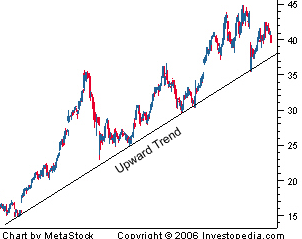
\includegraphics[keepaspectratio=true,scale=1]{figuras/up.png}
	\caption{Tendência de Subida \cite{investopedia}}
	\label{fig01}
\end{figure}

\begin{figure}[h]
	\centering
	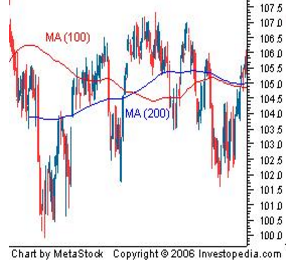
\includegraphics[keepaspectratio=true,scale=1]{figuras/flat.png}
	\caption{Tendência \cite{investopedia}}
	\label{fig02}
\end{figure}


\subsection{Suporte}

Níveis de suporte são níveis que históricamente os preços tem dificuldade em cair abaixo, agindo assim como uma linha de suporte.\cite{allen}

Na figura 03 pode-se perceber que ao longo do tempo, o preço da cotação apresentou certa resistência em ultrapassar o nível de suporte de 51.25

\begin{figure}[h]
	\centering
	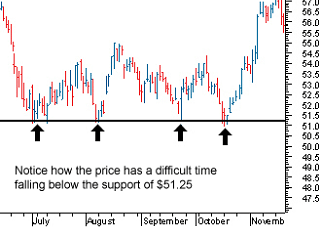
\includegraphics[keepaspectratio=true,scale=1]{figuras/sup.png}
	\caption{Suporte \cite{investopedia}}
	\label{fig03}
\end{figure}

\subsection{Resistência}

Níveis de resistência são exatamente o contrário de níveis de suporte, representando valores aos quais o preço históricamente tem dificuldade
em ultrapassar acima. O momento em que uma cotação ultrapassa uma linha de resistência é frequentemente chamado de breakout. \cite{allen}

\begin{figure}[h]
	\centering
	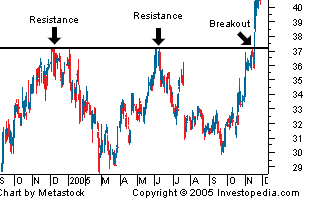
\includegraphics[keepaspectratio=true,scale=1]{figuras/resist.png}
	\caption{Resistência \cite{investopedia}}
	\label{fig04}
\end{figure}

\subsection{Indicadores}

Para entender os indicadores utilizados no Mercado de Moedas, é preciso saber que os preços são mostrados divididos em quatro valores:
\begin{itemize}
  \item Low: Menor cotação da moeda
  \item Open: Valor de entrada de acordo com a janela de tempo escolhida
  \item Close: Valor de fechamento de acordo com a janela de tempo escolhida
  \item High: Maior cotação da moeda
\end{itemize}

A figura 05 mostra um exemplo de como esses valores são evidenciados num gráfico do Mercado de Moedas

\begin{figure}[h]
	\centering
	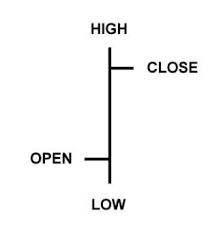
\includegraphics[keepaspectratio=true,scale=1]{figuras/data.png}
	\caption{Preço \cite{blue}}
	\label{fig05}
\end{figure}

Indicadores servem para processar esses valores de cotação e fornecer alguma perspectiva do mercado.

\subsubsection{Amplitude de Variação}

Um indicador simples e que fornece informação valiosa a respeito da volatilidade do mercado é a Amplitude de Variação, que nada mais é do que
a diferença entre a maior cotação da moeda e a menor cotação dessa mesma moeda para o mesmo período de tempo. \cite{investopedia}

% \begin{figure}[h]
% 	\centering
% 	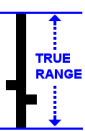
\includegraphics[keepaspectratio=true,scale=0.7]{figuras/true.png}
% 	\caption{Amplitude de Variação}
% 	\label{fig06}
% \end{figure}

A partir desse conceito
simples, é possível calcular a média da Amplitude de Variação para vários períodos de tempo. Por exemplo calculando essa média em um gráfico diário
com período de nove dias, é possível saber o quão volátil o mercado esteve nos 9 dias anteriores a cotação.

\subsubsection{Média Móvel}

Outro indicador comumente utilizado é a Média Móvel, que mostra o valor médio das cotações em um período de tempo específico,
ainda é possível atribuir coeficientes a essas cotações e atribuir um peso maior a cotações mais recentes por exemplo. Um exemplo de
Média Móvel pode ser visto na figura 07. \cite{investopedia}

\begin{figure}[h]
	\centering
	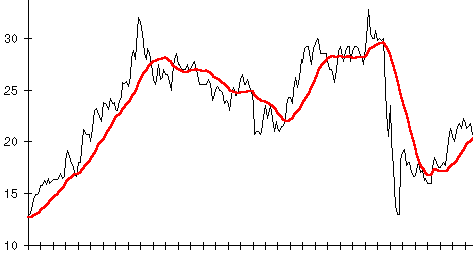
\includegraphics[keepaspectratio=true,scale=0.7]{figuras/mov.png}
	\caption{Média Móvel \cite{investopedia}}
	\label{fig07}
\end{figure}

\subsubsection{Estocástico}

Estocástico é um tipo de indicador cujo objetivo é comparar a cotação atual com as cotações anteriores durante um período de tempo determinado.
É baseado no pressuposto de que numa tendência de subida, os valores ficarão iguais ou maiores do que o valor anterior, já numa tendência
de queda, estes valores tendêm a permanecer iguais ou caírem. Utilizando uma escala para medir o grau de mudança entre cotações, este indicador tenta prever a probabilidade de continuação de tendência
do mercado. \cite{investopedia}

O oscilador estocástico apresenta duas linhas:

\begin{itemize}
  \item \%K - O atual valor de mercado
  \item \%D - É apresentado calculando a média móvel de \%K
\end{itemize}


\section{Redes Neurais}

O termo rede neural já é conhecido a algum tempo mas estas só começaram a ter grande impacto e impressionar com seus resultados
a pouco tempo. A razão disso é que quando as redes neurais foram inventadas ou primeiramente desenhadas, a tecnologia não apresentava
um grau de maturidade pronto para recebe-las e aplicá-las, principalmente porque para o bom funcionamento de uma rede neural, é preciso
um grande volume de dados e uma razoável capacidade de processamento. \cite{gross}

Com o grande avanço tecnológico, que é apresentado em várias vezes de forma exponencial, esse tema voltou a tona e agora com o poder de mostrar
muito mais do seu potencial.

\subsection{Neurociência}

O propósito das redes neurais é imitar o funcionamento do cerébro, que é uma das ferramentas mais fantásticas em termos de aprendizado.\cite{marilee}

Um cérebro humano possui cerca de cem bilhões de neurônios e cada um deles está conectado em aproximadamente outros mil neurônios próximos. \cite{kandel}
Na tentativa de imitar essa estrutura, uma rede neural artificial é composta de nós (neurônios). Esses nós são divididos em três camadas:

\begin{itemize}
	\item Camada de entrada: Onde váriaveis de entrada são captadas
	\item Camada de processamento: Onde os dados captados são processados
	\item Camada de saída: Onde os resultados obtidos são mostrados
\end{itemize}

\begin{figure}[h]
	\centering
	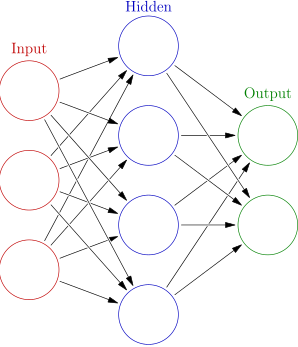
\includegraphics[keepaspectratio=true,scale=0.5]{figuras/neuron.png}
	\caption{Rede Neural \cite{glosser}}
	\label{fig08}
\end{figure}

O primeiro passo para criar uma rede neural é entender e imitar o funcionamento de um neurônio.

A figura 09 mostra como é a aparência de um neurônio:

\begin{figure}[h]
	\centering
	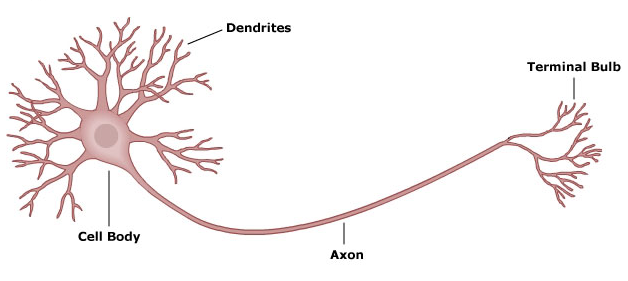
\includegraphics[keepaspectratio=true,scale=0.5]{figuras/n.png}
	\caption{Neurônio \cite{penn}}
	\label{fig09}
\end{figure}

Os vários ramos próximos ao corpo do neurônio são chamados dentritos e atuam como receptores, enquanto a extremidade longa do neurônio
é chamada de axônio e atua como um transmissor. Então atraves de uma conexão chamada synapse, os dentritos de um neurônio recebem sinais
dos axônios de outros neurônios. Então assim formando uma rede neural. \cite{kandel}

\subsection{Redes Neurais Artificiais}

Como visto anteriormente, redes neurais são formadas por três camadas (entrada, processamento e saída). A camada de entrada é formada
por váriaveis de entrada que são independentes, é importante que essas variáveis sejam padronizadas ou normalizadas antes de serem passadas
para a camada de processamento.\cite{levine}

Outra característica crucial para o funcionamento e aprendizado de uma rede neural é o conceito de pesos. Atribuindo pesos às entradas,
redes neurais conseguem decidir que entradas possuem maior ou menor relevância do que as outras, para cada nó de forma individual. Por exemplo
uma entrada pode ser importante para um nó específico e ser irrelevante para outro. São os pesos, as variáveis que são ajustadas durante
o processo de aprendizado de uma rede neural. \cite{yann}

Na camada de processamento, as váriaveis são somadas e processadas por uma função de ativação e enfim passadas para os próximos neurônios.

A camada de saída consiste na informação já processada pelos nós de processamento e é geralmente apresentada
das formas abaixo:

\begin{itemize}
	\item Forma contínua
	\item Forma binária
\end{itemize}

\subsection{Redes Neurais Recorrentes}

Redes neurais recorrentes são um tipo de rede neural artificial que busca imitar o lobo frontal do cérebro que dentre outras funções,
é responsável pela memória de curta duração.

\begin{figure}[h]
	\centering
	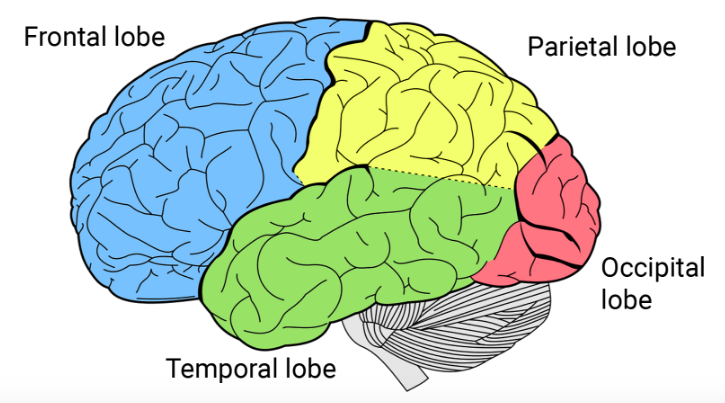
\includegraphics[keepaspectratio=true,scale=0.5]{figuras/brainn.png}
	\caption{Lobos Cerebrais \cite{queen}}
	\label{fig10}
\end{figure}

A grande diferença de redes neurais recorrentes para os outros tipos de redes neurais é o chamado "loop temporal". Cada nó de processamento
não só passa suas saída para os outros nós como também para si mesmo, sua saída também serve de entrada para si próprio. \cite{jaeger}

A figura 11 busca retratar o loop temporal:

\begin{figure}[h]
	\centering
	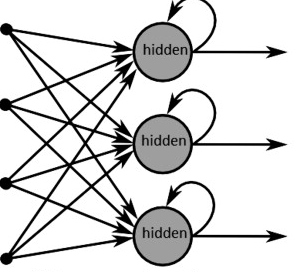
\includegraphics[keepaspectratio=true,scale=0.5]{figuras/rnn.png}
	\caption{Loop Temporal}
	\label{fig11}
\end{figure}

O loop temporal permite que um nó tenha uma memória de curta duração, sabendo o valor que foi processado nele anteriormente.
